\documentclass[a4 paper]{article}
\usepackage[inner=2.0cm,outer=2.0cm,top=2.5cm,bottom=2.5cm]{geometry}
\usepackage{setspace}
\usepackage[rgb]{xcolor}
\usepackage{verbatim}
\usepackage{subcaption}
\usepackage{amsgen,amsmath,amstext,amsbsy,amsopn,tikz,amssymb}
\usepackage{fancyhdr}
\usepackage[colorlinks=true, urlcolor=blue,  linkcolor=blue, citecolor=blue]{hyperref}
\usepackage[colorinlistoftodos]{todonotes}
\usepackage{rotating}
\usepackage{booktabs}
\newcommand{\ra}[1]{\renewcommand{\arraystretch}{#1}}
\usepackage{algorithmic}

\newtheorem{thm}{Theorem}[section]
\newtheorem{prop}[thm]{Proposition}
\newtheorem{lem}[thm]{Lemma}
\newtheorem{cor}[thm]{Corollary}
\newtheorem{defn}[thm]{Definition}
\newtheorem{rem}[thm]{Remark}
\numberwithin{equation}{section}

\newcommand{\homework}[6]{
   \pagestyle{myheadings}
   \thispagestyle{plain}
   \newpage
   \setcounter{page}{1}
   \noindent
   \begin{center}
   \framebox{
      \vbox{\vspace{2mm}
    \hbox to 6.28in { {\bf CSE 211:~Discrete Mathematics \hfill {\small (#2)}} }
       \vspace{6mm}
       \hbox to 6.28in { {\Large \hfill #1  \hfill} }
       \vspace{6mm}
       \hbox to 6.28in { {\it Instructor: {\rm #3} \hfill  {\rm #5} \hfill  {\rm #6}} \hfill}
       \hbox to 6.28in { {\it Assistant: #4  \hfill #6}}
      \vspace{2mm}}
   }
   \end{center}
   \markboth{#5 -- #1}{#5 -- #1}
   \vspace*{4mm}
}

\newcommand{\problem}[2]{~\\\fbox{\textbf{Problem #1}}\hfill (#2 points)\newline\newline}
\newcommand{\subproblem}[1]{~\newline\textbf{(#1)}}
\newcommand{\D}{\mathcal{D}}
\newcommand{\Hy}{\mathcal{H}}
\newcommand{\VS}{\textrm{VS}}
\newcommand{\solution}{~\newline\textbf{\textit{(Solution)}} }

\newcommand{\bbF}{\mathbb{F}}
\newcommand{\bbX}{\mathbb{X}}
\newcommand{\bI}{\mathbf{I}}
\newcommand{\bX}{\mathbf{X}}
\newcommand{\bY}{\mathbf{Y}}
\newcommand{\bepsilon}{\boldsymbol{\epsilon}}
\newcommand{\balpha}{\boldsymbol{\alpha}}
\newcommand{\bbeta}{\boldsymbol{\beta}}
\newcommand{\0}{\mathbf{0}}


\begin{document}
\homework{Homework \#1}{Due: 17/11/20}{Dr. Zafeirakis Zafeirakopoulos}{Gizem S\"ung\"u}{}{}
\textbf{Course Policy}: Read all the instructions below carefully before you start working on the assignment, and before you make a submission.
\begin{itemize}
\item It is not a group homework. Do not share your answers to anyone in any circumstance. Any cheating means at least -100 for both sides. 
\item Do not take any information from Internet.
\item No late homework will be accepted. 
\item For any questions about the homework, send an email to gizemsungu@gtu.edu.tr
\item The homeworks (both latex and pdf files in a zip file) will be
submitted into the course page of Moodle.
\item The latex, pdf and zip files of the homeworks should be saved as
"Name\_Surname\_StudentId".$\{$tex, pdf, zip$\}$.
\item If the answers of the homeworks have only calculations without any formula or any explanation -when needed- will get zero.
\item Writing the homeworks on Latex is strongly suggested. However, hand-written paper is still accepted $\textbf{IFF}$ hand writing of the student is clear and understandable to read, and the paper is well-organized. Otherwise, the assistant cannot grade the student's homework.
\end{itemize}

\problem{1: Conditional Statements}{5+5+5=15}
State the converse, contrapositive, and inverse of each of these conditional statements.

\subproblem{a} If it snows tonight, then I will stay at home.
\solution
\newline
\newline
\textbf{Converse:}
If I will stay at home, then it snows tonight.
\newline
\newline
\textbf{Contrapositive:}
If I will not stay at home, then it does not snow tonight.
\newline
\newline
\textbf{Inverse:}
If it does not snow tonight, then I will not stay at home.
\newline

\subproblem{b} I go to the beach whenever it is a sunny summer day.
\solution
\newline
\newline
\textbf{Converse:}
It is a sunny summer day whenever I go to the beach.
\newline
\newline
\textbf{Contrapositive:}
It is not a sunny summer day whenever I do not go to the beach.
\newline
\newline
\textbf{Inverse:}
I do not go to the beach whenever it is not is a sunny summer day.
\newline

\newpage
\subproblem{c} If I stay up late, then I sleep until noon.
\solution
\newline
\newline
\textbf{Converse:}
If I sleep until noon, then I stay up late.
\newline
\newline
\textbf{Contrapositive:}
If I do not sleep until noon, then I do not stay up late.
\newline
\newline
\textbf{Inverse:}
If I do not stay up late, then I do not sleep until noon.
\newline
\newline

\problem{2: Truth Tables For Logic Operators}{5+5+5=15}
Construct a truth table for each of the following compound propositions.
\subproblem{a} (p $\oplus$ $\neg$ q)
\solution

\begin{table}[h]
\begin{tabular}{c|c|c|c}
\textbf{p} & \textbf{q} & \textbf{$\neg$ q} & \textbf{p $\oplus$ $\neg$ q} \\ \hline
0 & 0 & 1 & 1 \\
0 & 1 & 0 & 0 \\
1 & 0 & 1 & 0 \\
1 & 1 & 0 & 1 
\end{tabular}
\end{table}

\subproblem{b} (p $\iff$ q) $\oplus$ ( $\neg$ p $\iff$ $\neg$ r)
\solution 

\begin{table}[h]
\begin{tabular}{c|c|c|c|c|c|c|c}
\textbf{p} & \textbf{q} & \textbf{r} & \textbf{$\neg$ p} & \textbf{$\neg$ r} & \textbf{p $\iff$ q} & \textbf{$\neg$ p $\iff$ $\neg$ r} & \textbf{(p $\iff$ q) $\oplus$ ($\neg$ p $\iff$ $\neg$ r)} \\ \hline
0 & 0 & 0 & 1 & 1 & 1 & 1 & 0\\
0 & 0 & 1 & 1 & 0 & 1 & 0 & 1\\
0 & 1 & 0 & 1 & 1 & 0 & 1 & 1\\
0 & 1 & 1 & 1 & 0 & 0 & 0 & 0\\
1 & 0 & 0 & 0 & 1 & 0 & 0 & 0\\
1 & 0 & 1 & 0 & 0 & 0 & 1 & 1\\
1 & 1 & 0 & 0 & 1 & 1 & 0 & 1\\
1 & 1 & 1 & 0 & 0 & 1 & 1 & 0
\end{tabular}
\end{table}

\subproblem{c} (p $\oplus$ q) $\Rightarrow$ (p $\oplus$ $\neg$ q)
\solution

\begin{table}[h]
\begin{tabular}{c|c|c|c|c|c}
\textbf{p} & \textbf{q} & \textbf{$\neg$ q} & \textbf{p $\oplus$ q} & \textbf{p $\oplus$ $\neg$ q} & \textbf{(p $\oplus$ q) $\Rightarrow$ (p $\oplus$ $\neg$ q)} \\ \hline
0 & 0 & 1 & 0 & 1 & 1\\
0 & 1 & 0 & 1 & 0 & 0\\
1 & 0 & 1 & 1 & 0 & 0\\
1 & 1 & 0 & 0 & 1 & 1
\end{tabular}
\end{table}

\newpage
\problem{3: Predicates and Quantifiers}{21}
There are three predicate logic statements which represent English sentences as follows.
\begin{itemize}
	\item P(x): "x can speak English."
	\item Q(x): "x knows Python."
	\item H(x): "x is happy."
\end{itemize}
Express each of the following sentences in terms of P(x), Q(x), H(x), quantifiers, and logical connectives or vice versa. The domain
for quantifiers consists of all students at the university.
\subproblem{a} There is a student at the university who can speak English and who knows Python.
\solution
\newline
\newline
$\exists$x ( P(x) $\wedge$ Q(x) )
\newline
\subproblem{b} There is a student at the university who can speak English but who doesn’t know Python.
\solution
\newline
\newline
$\exists$x ( P(x) $\wedge$ $\neg$ Q(x) )
\newline
\subproblem{c} Every student at the university either can speak English or knows Python.
\solution
\newline
\newline
Either or means that p or q not both. \newline
$\forall$x ( P(x) $\oplus$ Q(x) )
\newline
\subproblem{d} No student at the university can speak English or knows Python.
\solution
\newline
\newline
This means that everyone at the university can not speak English and does not know Python.
\newline
$\neg$ $\exists$x ( P(x) $\vee$ Q(x) ) = $\forall$x ( $\neg$ P(x) $\wedge$ $\neg$ Q(x) )
\newline
\subproblem{e} If there is a student at the university who can speak English and know Python, then she/he is happy.
\solution
\newline
\newline
$\exists$x ( (P(x) $\wedge$ Q(x)) $\Rightarrow$ H(x) )
\newline
\subproblem{f} At least two students are happy.
\solution
\newline
\newline
$\exists$x$\exists$y ( H(x) $\wedge$ H(y) )
\newline
\subproblem{g} $\neg \forall x (Q(x) \wedge P(x))$
\solution
\newline
\newline
Negation of "Every student at the university knows Python and can speak English."
\newline
Not every student at the university knows Python and can speak English.
\newpage

\problem{4: Mathematical Induction}{21}
Prove that 3 + 3 . 5 + 3 . $5^2$ + . . . + 3 . $5^n$ =$\frac{3(5^{n+1} - 1)}{4}$
whenever n is a nonnegative integer.
\solution
\newline
\newline
n $>$ 0 and n $\in$ Z \newline \newline
\textbf{Basis Step:} \newline
Let n = 1, then 3 . $5^0$ + 3 . $5^1$ = $\frac{3(5^{1+1}-1)}{4}$
\newline
3 . 1 + 3 . 5 = $\frac{3 . 24}{4}$ is correct.
\newline
We show that the basis step is correct when n = 1. \newline \newline
\textbf{Inductive Step:} \newline
Let n = k, then we accept that \newline
3 . $5^0$ + 3 . $5^1$ + 3 . $5^2$ + . . . +  3 . $5^k$ = $\frac{3(5^{k+1} - 1)}{4}$ = a is correct. \newline \newline
Let n = k + 1, then we have to prove that\newline
3 . $5^0$ + 3 . $5^1$ + 3 . $5^2$ + . . . +  3 . $5^k$ + 3 . $5^{k+1}$ = $\frac{3(5^{k+1+1} - 1)}{4}$ is correct. \newline \newline
Instead of part a in the equation above, we can write the right hand side of the equation for n = k. Hence \newline
$\frac{3(5^{k+1} - 1)}{4}$ + 3 . $5^{k+1}$ = $\frac{3(5^{k+2}-1)}{4}$ \newline \newline
Multiply both sides of the equation by 4 \newline
3($5^{k+1}$ - 1) + 12 . $5^{k+1}$ = 3($5^{k+2}$ - 1) \newline \newline
After some operations \newline
3 . $5^{k+1}$ - 3 + 12 . $5^{k+1}$ = 3 . $5^{k+2}$ - 3 \newline
15 . $5^{k+1}$ = 3 . $5^{k+2}$ \newline
3 . 5 . $5^{k+1}$ = 3 . $5^{k+2}$ \newline
3 . $5^{k+2}$ = 3 . $5^{k+2}$ \newline \newline
So we prove that 3 + 3 . 5 + 3 . $5^2$ + . . . + 3 . $5^n$ =$\frac{3(5^{n+1} - 1)}{4}$ is true when n is a nonnegative integer.
\newline
\problem{5: Mathematical Induction}{20}
Prove that $n^2$ - 1 is divisible by 8 whenever n is an odd
positive integer.
\solution
\newline
\newline
\textbf{Basis Step:} \newline
Let n = 1, then $1^1$ - 1 = 0 is divisible by 8. \newline
We show that the statement is correct in the basis step when n = 1. \newline \newline
\textbf{Inductive Step:} \newline
Let n = 2k + 1, k is nonnegative integer, then we accept that $(2k + 1)^2$ - 1 is divisible by 8 is correct. \newline
$(2k + 1)^2$ - 1 = 4$k^2$ + 4k + 1 - 1 = 4$k^2$ + 4k is divisible by 8. \newline \newline
Let n = 2k + 3, because k should be odd positive integer and we should increase by 2 to provide domain, then we have to prove that $(2k + 3)^2$ - 1 is divisible by 8 is correct. \newline \newline
$(2k + 3)^2$ - 1 = $4k^2$ + 12k + 9 - 1 \newline
$4k^2$ + 12k + 9 - 1 = $4k^2$ + 4k + 8k + 8 = $4k^2$ + 4k + 8(k + 1) \newline
We know that $4k^2$ + 4k is divisible by 8 and 8(k + 1) is divisible by 8. \newline
So we prove that $n^2$ - 1 is divisible by 8 whenever n is an odd positive integer. \newline
\newpage
\problem{6: Sets}{8}
Which of the following sets are equal? Show your work step by step.\newline
\subproblem{a} $\{$t : t is a root of $x^2$ – 6x + 8 = 0$\}$
\newline
\subproblem{b} $\{$y : y is a real number in the closed interval [2, 3]$\}$
\newline
\subproblem{c} $\{$4, 2, 5, 4$\}$
\newline
\subproblem{d} $\{$4, 5, 7, 2$\}$ - $\{$5, 7$\}$
\newline
\subproblem{e} $\{$q: q is either the number of sides of a rectangle or the number of digits in any integer between 11 and 99$\}$\\
\solution \newline
\subproblem{a} $x^2$ - 6x + 8 = 0 \newline
(x - 4)(x - 2) = 0\newline
x = 4, x = 2 \newline
A = $\{$4, 2$\}$ \newline
\subproblem{b} B = $\{$2, ..., 3$\}$, s(B) = $\infty$ \newline
\subproblem{c} The elements of a set should be distinct. So, if any element of a set is repeated number of times in the set, we consider it as a single element. Thus, $\{$1, 1, 2, 2, 3, 3, 4, 4, 4$\}$ = $\{$1, 2, 3, 4$\}$ \newline
C = $\{$4, 2, 5, 4$\}$ = $\{$4, 2, 5$\}$ \newline
\subproblem{d} D = $\{$4, 5, 7, 2$\}$ - $\{$5, 7$\}$ = $\{$4, 2$\}$ \newline
\subproblem{e}
Number of sides of a rectangle is a 4. All integers between 11 and 99 have 2 digits.\newline
E = $\{$4, 2$\}$ \newline \newline
We know that the order of the elements in sets does not matter.\newline
In order for two sets to be equal, their elements must be exactly the same and the number of elements must be the same. \newline
A = $\{$4, 2$\}$ \newline
D = $\{$4, 2$\}$ \newline
E = $\{$4, 2$\}$ \newline
s(A) = s(D) = s(E) = 2, A = D = E \newline
\newpage
\problem{Bonus: Logic in Algorithms}{20}
Let p and q be the statements as follows.
\begin{itemize}
	\item $\textbf{p:}$ It is sunny.
	\item $\textbf{q:}$ The flowers are blooming.
\end{itemize}
\begin{figure*}[htp]
	\centering
	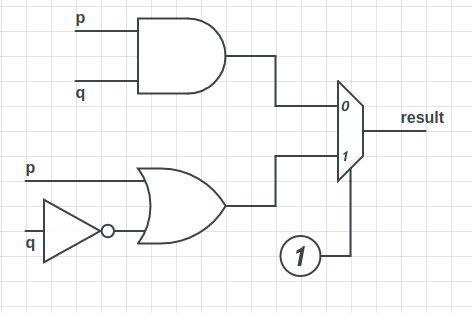
\includegraphics[scale=0.5]{circuit.png}
	\caption{Combinational Circuit}
	\label{fig: circuit}
	
\end{figure*}
In Figure \ref{fig: circuit}, the two statements are used as input. The circuit has 3 gates as AND, OR and NOT operators. It has also a 2x1 multiplexer\footnote{https://www.geeksforgeeks.org/multiplexers-in-digital-logic/} which provides to select one of the two options. 
\subproblem{a} Write the sentence that "result" output has.
\solution\newline\newline
1 is selected in the multiplexor. This means that the expression p $\vee$ $\neg$ q is selected.\newline
p $\vee$ $\neg$ q $\equiv$ $\neg$ q $\vee$ p $\equiv$ q $\Rightarrow$ p \newline
Result is "If the flowers are blooming, then it is sunny".\newline
\subproblem{b} Convert Figure \ref{fig: circuit} to an algorithm which you can write in any programming language that you prefer (including pseudocode).
\solution \newline
\begin{algorithmic}
\IF{0 is selected in the multiplexor}
\STATE print "It is sunny and the flowers are blooming"
\ELSE
\STATE print "If the flowers are blooming, then it is sunny"
\ENDIF
\end{algorithmic}
\end{document}